% Options for packages loaded elsewhere
% Options for packages loaded elsewhere
\PassOptionsToPackage{unicode}{hyperref}
\PassOptionsToPackage{hyphens}{url}
\PassOptionsToPackage{dvipsnames,svgnames,x11names}{xcolor}
%
\documentclass[
  12pt,
]{article}
\usepackage{xcolor}
\usepackage[margin=2cm]{geometry}
\usepackage{amsmath,amssymb}
\setcounter{secnumdepth}{5}
\usepackage{iftex}
\ifPDFTeX
  \usepackage[T1]{fontenc}
  \usepackage[utf8]{inputenc}
  \usepackage{textcomp} % provide euro and other symbols
\else % if luatex or xetex
  \usepackage{unicode-math} % this also loads fontspec
  \defaultfontfeatures{Scale=MatchLowercase}
  \defaultfontfeatures[\rmfamily]{Ligatures=TeX,Scale=1}
\fi
\usepackage{lmodern}
\ifPDFTeX\else
  % xetex/luatex font selection
  \setmainfont[]{Times New Roman}
\fi
% Use upquote if available, for straight quotes in verbatim environments
\IfFileExists{upquote.sty}{\usepackage{upquote}}{}
\IfFileExists{microtype.sty}{% use microtype if available
  \usepackage[]{microtype}
  \UseMicrotypeSet[protrusion]{basicmath} % disable protrusion for tt fonts
}{}
\usepackage{setspace}
\makeatletter
\@ifundefined{KOMAClassName}{% if non-KOMA class
  \IfFileExists{parskip.sty}{%
    \usepackage{parskip}
  }{% else
    \setlength{\parindent}{0pt}
    \setlength{\parskip}{6pt plus 2pt minus 1pt}}
}{% if KOMA class
  \KOMAoptions{parskip=half}}
\makeatother
% Make \paragraph and \subparagraph free-standing
\makeatletter
\ifx\paragraph\undefined\else
  \let\oldparagraph\paragraph
  \renewcommand{\paragraph}{
    \@ifstar
      \xxxParagraphStar
      \xxxParagraphNoStar
  }
  \newcommand{\xxxParagraphStar}[1]{\oldparagraph*{#1}\mbox{}}
  \newcommand{\xxxParagraphNoStar}[1]{\oldparagraph{#1}\mbox{}}
\fi
\ifx\subparagraph\undefined\else
  \let\oldsubparagraph\subparagraph
  \renewcommand{\subparagraph}{
    \@ifstar
      \xxxSubParagraphStar
      \xxxSubParagraphNoStar
  }
  \newcommand{\xxxSubParagraphStar}[1]{\oldsubparagraph*{#1}\mbox{}}
  \newcommand{\xxxSubParagraphNoStar}[1]{\oldsubparagraph{#1}\mbox{}}
\fi
\makeatother

\usepackage{color}
\usepackage{fancyvrb}
\newcommand{\VerbBar}{|}
\newcommand{\VERB}{\Verb[commandchars=\\\{\}]}
\DefineVerbatimEnvironment{Highlighting}{Verbatim}{commandchars=\\\{\}}
% Add ',fontsize=\small' for more characters per line
\usepackage{framed}
\definecolor{shadecolor}{RGB}{241,243,245}
\newenvironment{Shaded}{\begin{snugshade}}{\end{snugshade}}
\newcommand{\AlertTok}[1]{\textcolor[rgb]{0.68,0.00,0.00}{#1}}
\newcommand{\AnnotationTok}[1]{\textcolor[rgb]{0.37,0.37,0.37}{#1}}
\newcommand{\AttributeTok}[1]{\textcolor[rgb]{0.40,0.45,0.13}{#1}}
\newcommand{\BaseNTok}[1]{\textcolor[rgb]{0.68,0.00,0.00}{#1}}
\newcommand{\BuiltInTok}[1]{\textcolor[rgb]{0.00,0.23,0.31}{#1}}
\newcommand{\CharTok}[1]{\textcolor[rgb]{0.13,0.47,0.30}{#1}}
\newcommand{\CommentTok}[1]{\textcolor[rgb]{0.37,0.37,0.37}{#1}}
\newcommand{\CommentVarTok}[1]{\textcolor[rgb]{0.37,0.37,0.37}{\textit{#1}}}
\newcommand{\ConstantTok}[1]{\textcolor[rgb]{0.56,0.35,0.01}{#1}}
\newcommand{\ControlFlowTok}[1]{\textcolor[rgb]{0.00,0.23,0.31}{\textbf{#1}}}
\newcommand{\DataTypeTok}[1]{\textcolor[rgb]{0.68,0.00,0.00}{#1}}
\newcommand{\DecValTok}[1]{\textcolor[rgb]{0.68,0.00,0.00}{#1}}
\newcommand{\DocumentationTok}[1]{\textcolor[rgb]{0.37,0.37,0.37}{\textit{#1}}}
\newcommand{\ErrorTok}[1]{\textcolor[rgb]{0.68,0.00,0.00}{#1}}
\newcommand{\ExtensionTok}[1]{\textcolor[rgb]{0.00,0.23,0.31}{#1}}
\newcommand{\FloatTok}[1]{\textcolor[rgb]{0.68,0.00,0.00}{#1}}
\newcommand{\FunctionTok}[1]{\textcolor[rgb]{0.28,0.35,0.67}{#1}}
\newcommand{\ImportTok}[1]{\textcolor[rgb]{0.00,0.46,0.62}{#1}}
\newcommand{\InformationTok}[1]{\textcolor[rgb]{0.37,0.37,0.37}{#1}}
\newcommand{\KeywordTok}[1]{\textcolor[rgb]{0.00,0.23,0.31}{\textbf{#1}}}
\newcommand{\NormalTok}[1]{\textcolor[rgb]{0.00,0.23,0.31}{#1}}
\newcommand{\OperatorTok}[1]{\textcolor[rgb]{0.37,0.37,0.37}{#1}}
\newcommand{\OtherTok}[1]{\textcolor[rgb]{0.00,0.23,0.31}{#1}}
\newcommand{\PreprocessorTok}[1]{\textcolor[rgb]{0.68,0.00,0.00}{#1}}
\newcommand{\RegionMarkerTok}[1]{\textcolor[rgb]{0.00,0.23,0.31}{#1}}
\newcommand{\SpecialCharTok}[1]{\textcolor[rgb]{0.37,0.37,0.37}{#1}}
\newcommand{\SpecialStringTok}[1]{\textcolor[rgb]{0.13,0.47,0.30}{#1}}
\newcommand{\StringTok}[1]{\textcolor[rgb]{0.13,0.47,0.30}{#1}}
\newcommand{\VariableTok}[1]{\textcolor[rgb]{0.07,0.07,0.07}{#1}}
\newcommand{\VerbatimStringTok}[1]{\textcolor[rgb]{0.13,0.47,0.30}{#1}}
\newcommand{\WarningTok}[1]{\textcolor[rgb]{0.37,0.37,0.37}{\textit{#1}}}

\usepackage{longtable,booktabs,array}
\newcounter{none} % for unnumbered tables
\usepackage{calc} % for calculating minipage widths
% Correct order of tables after \paragraph or \subparagraph
\usepackage{etoolbox}
\makeatletter
\patchcmd\longtable{\par}{\if@noskipsec\mbox{}\fi\par}{}{}
\makeatother
% Allow footnotes in longtable head/foot
\IfFileExists{footnotehyper.sty}{\usepackage{footnotehyper}}{\usepackage{footnote}}
\makesavenoteenv{longtable}
\usepackage{graphicx}
\makeatletter
\newsavebox\pandoc@box
\newcommand*\pandocbounded[1]{% scales image to fit in text height/width
  \sbox\pandoc@box{#1}%
  \Gscale@div\@tempa{\textheight}{\dimexpr\ht\pandoc@box+\dp\pandoc@box\relax}%
  \Gscale@div\@tempb{\linewidth}{\wd\pandoc@box}%
  \ifdim\@tempb\p@<\@tempa\p@\let\@tempa\@tempb\fi% select the smaller of both
  \ifdim\@tempa\p@<\p@\scalebox{\@tempa}{\usebox\pandoc@box}%
  \else\usebox{\pandoc@box}%
  \fi%
}
% Set default figure placement to htbp
\def\fps@figure{htbp}
\makeatother


% definitions for citeproc citations
\NewDocumentCommand\citeproctext{}{}
\NewDocumentCommand\citeproc{mm}{%
  \begingroup\def\citeproctext{#2}\cite{#1}\endgroup}
\makeatletter
 % allow citations to break across lines
 \let\@cite@ofmt\@firstofone
 % avoid brackets around text for \cite:
 \def\@biblabel#1{}
 \def\@cite#1#2{{#1\if@tempswa , #2\fi}}
\makeatother
\newlength{\cslhangindent}
\setlength{\cslhangindent}{1.5em}
\newlength{\csllabelwidth}
\setlength{\csllabelwidth}{3em}
\newenvironment{CSLReferences}[2] % #1 hanging-indent, #2 entry-spacing
 {\begin{list}{}{%
  \setlength{\itemindent}{0pt}
  \setlength{\leftmargin}{0pt}
  \setlength{\parsep}{0pt}
  % turn on hanging indent if param 1 is 1
  \ifodd #1
   \setlength{\leftmargin}{\cslhangindent}
   \setlength{\itemindent}{-1\cslhangindent}
  \fi
  % set entry spacing
  \setlength{\itemsep}{#2\baselineskip}}}
 {\end{list}}
\usepackage{calc}
\newcommand{\CSLBlock}[1]{\hfill\break\parbox[t]{\linewidth}{\strut\ignorespaces#1\strut}}
\newcommand{\CSLLeftMargin}[1]{\parbox[t]{\csllabelwidth}{\strut#1\strut}}
\newcommand{\CSLRightInline}[1]{\parbox[t]{\linewidth - \csllabelwidth}{\strut#1\strut}}
\newcommand{\CSLIndent}[1]{\hspace{\cslhangindent}#1}



\setlength{\emergencystretch}{3em} % prevent overfull lines

\providecommand{\tightlist}{%
  \setlength{\itemsep}{0pt}\setlength{\parskip}{0pt}}



 


\usepackage{booktabs}
\usepackage{longtable}
\usepackage{array}
\usepackage{multirow}
\usepackage{wrapfig}
\usepackage{float}
\usepackage{colortbl}
\usepackage{pdflscape}
\usepackage{tabu}
\usepackage{threeparttable}
\usepackage{threeparttablex}
\usepackage[normalem]{ulem}
\usepackage{makecell}
\usepackage{xcolor}
\usepackage[noblocks]{authblk}
\renewcommand*{\Authsep}{, }
\renewcommand*{\Authand}{, }
\renewcommand*{\Authands}{, }
\renewcommand\Affilfont{\small}
\makeatletter
\@ifpackageloaded{tcolorbox}{}{\usepackage[skins,breakable]{tcolorbox}}
\@ifpackageloaded{fontawesome5}{}{\usepackage{fontawesome5}}
\definecolor{quarto-callout-color}{HTML}{909090}
\definecolor{quarto-callout-note-color}{HTML}{0758E5}
\definecolor{quarto-callout-important-color}{HTML}{CC1914}
\definecolor{quarto-callout-warning-color}{HTML}{EB9113}
\definecolor{quarto-callout-tip-color}{HTML}{00A047}
\definecolor{quarto-callout-caution-color}{HTML}{FC5300}
\definecolor{quarto-callout-color-frame}{HTML}{acacac}
\definecolor{quarto-callout-note-color-frame}{HTML}{4582ec}
\definecolor{quarto-callout-important-color-frame}{HTML}{d9534f}
\definecolor{quarto-callout-warning-color-frame}{HTML}{f0ad4e}
\definecolor{quarto-callout-tip-color-frame}{HTML}{02b875}
\definecolor{quarto-callout-caution-color-frame}{HTML}{fd7e14}
\makeatother
\makeatletter
\@ifpackageloaded{caption}{}{\usepackage{caption}}
\AtBeginDocument{%
\ifdefined\contentsname
  \renewcommand*\contentsname{Table of contents}
\else
  \newcommand\contentsname{Table of contents}
\fi
\ifdefined\listfigurename
  \renewcommand*\listfigurename{List of Figures}
\else
  \newcommand\listfigurename{List of Figures}
\fi
\ifdefined\listtablename
  \renewcommand*\listtablename{List of Tables}
\else
  \newcommand\listtablename{List of Tables}
\fi
\ifdefined\figurename
  \renewcommand*\figurename{Figure}
\else
  \newcommand\figurename{Figure}
\fi
\ifdefined\tablename
  \renewcommand*\tablename{Table}
\else
  \newcommand\tablename{Table}
\fi
}
\@ifpackageloaded{float}{}{\usepackage{float}}
\floatstyle{ruled}
\@ifundefined{c@chapter}{\newfloat{codelisting}{h}{lop}}{\newfloat{codelisting}{h}{lop}[chapter]}
\floatname{codelisting}{Listing}
\newcommand*\listoflistings{\listof{codelisting}{List of Listings}}
\makeatother
\makeatletter
\makeatother
\makeatletter
\@ifpackageloaded{caption}{}{\usepackage{caption}}
\@ifpackageloaded{subcaption}{}{\usepackage{subcaption}}
\makeatother
\usepackage{bookmark}
\IfFileExists{xurl.sty}{\usepackage{xurl}}{} % add URL line breaks if available
\urlstyle{same}
\hypersetup{
  pdftitle={Redistributive Justice{,} Job Insecurity{,} and Perceived Technological Risk: How Labor Market Position Shapes the Legitimacy of the Welfare State in 27 OECD Countries},
  pdfauthor={Kevin Carrasco},
  colorlinks=true,
  linkcolor={blue},
  filecolor={Maroon},
  citecolor={Blue},
  urlcolor={Blue},
  pdfcreator={LaTeX via pandoc}}


\title{Redistributive Justice, Job Insecurity, and Perceived
Technological Risk: How Labor Market Position Shapes the Legitimacy of
the Welfare State in 27 OECD Countries}


  \author{Kevin Carrasco}
            \affil{%
                  Nucleo Milenio sobre Evolución del Trabajo (M-new)
              }
      
\date{}
\begin{document}
\maketitle
\begin{abstract}
This study \newline \textbf{Keywords}: Redistributive preferences, Labor
market position, Welfare State
\end{abstract}


\setstretch{1.15}
\section{Introduction}\label{introduction}

Contemporary technological transformations, such as automation,
artificial intelligence, algorithmic management and intermediation
through digital platforms, are altering the conditions under which
workers relate to social protection systems
(\citeproc{ref-frey_future_2017}{Frey and Osborne, 2017};
\citeproc{ref-vallas_what_2020}{Vallas and Schor, 2020}). What is
sometimes termed the fourth industrial revolution changes the content of
tasks and the stability of employment, the subjective experience that
workers have of their position in the labour market and, with it, their
assessment of the fairness of their relationship with the welfare state
(\citeproc{ref-busemeyer_social_2022}{Busemeyer and Sahm, 2022};
\citeproc{ref-gallego_automation_2022}{Gallego and Kurer, 2022}). These
systems were built on the premise of stable, full-time and long-term
employment, in which contributions flowed predictably from wages and
rights accumulated over continuous careers
(\citeproc{ref-esping-andersen_three_1993}{Esping-Andersen, 1993};
\citeproc{ref-korpi_paradox_1998}{Korpi and Palme, 1998}). The
progressive decoupling between that model and the actual forms of work,
mainly through temporary contracts, self-employment and
platform-mediated work, raises the question of how citizens today
perceive the fairness of the exchange they maintain with the
institutions that ought to protect them.

Research on attitudes towards the welfare state has examined extensively
the determinants of support for redistribution, showing that exposure to
labour market risk and to automation tends to increase the demand for
social protection (\citeproc{ref-busemeyer_social_2022}{Busemeyer and
Sahm, 2022}; \citeproc{ref-rehm_risks_2009}{Rehm, 2009};
\citeproc{ref-thewissen_automation_2019}{Thewissen and Rueda, 2019}).
Much less attention has been paid, by contrast, to perceived
redistributive justice, that is, to the evaluative judgement of whether
the benefits that an individual receives from the state constitute fair
compensation for the taxes and contributions they pay
(\citeproc{ref-roosma_just_2016}{Roosma et al., 2016}).

This study addresses whether perceiving the functioning of the state as
fair is related to labour market position and the perception of
technological risk. Drawing on data from the Risks That Matter survey of
the OECD (2024), which covers more than 40,000 people in 27 countries,
this research simultaneously introduces three little-explored elements.
First, it distinguishes labour market position according to type of
employment ---formal employees, self-employed workers and platform
workers---, forms that maintain unequal links with the social protection
system and that have rarely been examined together in relation to
perceived redistributive justice. Second, it incorporates the perception
of technological risk as a source of redistributive dissatisfaction
distinct from type of employment and from conventional job insecurity,
distinguishing its threatening dimension ---the likelihood of being
displaced by automation, artificial intelligence, platform competition
or the obsolescence of one's own skills--- from its enabling dimension
---the perception that technology can improve working conditions---.
Third, it incorporates the perceived deservingness of others ---the
judgement of whether others receive benefits from the state that they do
not deserve--- as a predictor of the assessment that each individual
makes of their own relationship with the system
(\citeproc{ref-vanoorschot_making_2006}{Van Oorschot, 2006},
\citeproc{ref-oorschot_who_2000}{2000}).

The study makes three contributions. First, it extends the sociology of
welfare attitudes by situating the structural conditions of the labour
market as explanatory variables of perceived redistributive justice,
linking subjective assessments with the organisation of work
(\citeproc{ref-emmenegger_age_2012}{Emmenegger et al., 2012};
\citeproc{ref-kalleberg_good_2011}{Kalleberg, 2011}). Second, it
provides comparative evidence on the effect of the perception of
technological risk in an attitudinal domain distinct from the one that
recent literature has concentrated on, concerned above all with support
for redistribution or for social investment
(\citeproc{ref-busemeyer_social_2022}{Busemeyer and Sahm, 2022};
\citeproc{ref-thewissen_automation_2019}{Thewissen and Rueda, 2019}).
Third, it places these processes within a comparative framework of
welfare regimes, which makes it possible to assess how different
institutional contexts moderate the relationship between labour market
vulnerability, technological perception and judgements of fairness
(\citeproc{ref-esping-andersen_three_1993}{Esping-Andersen, 1993};
\citeproc{ref-larsen_institutional_2008}{Larsen, 2008}).

The argument organising this work is that the perception of fairness in
the relationship between what one contributes and what one receives is
not solely a function of ideological predispositions or of abstract
beliefs about inequality, but is anchored in the everyday experience of
workers in the labour market, that is, the employment relationship
through which they are linked to the protection system, how secure they
feel in their jobs, whether they perceive technology as a threat or as
an opportunity, and how they judge the deservingness of those who also
receive from the state. Although the welfare state was designed for a
world of stable employment, its perceived legitimacy is called into
question by labour markets that increasingly depart from that
foundational assumption
(\citeproc{ref-howcroft_digitalisation_2025}{Howcroft et al., 2025};
\citeproc{ref-standing_precariat_2014}{Standing, 2014}).

\subsection{Redistributive justice as
reciprocity}\label{redistributive-justice-as-reciprocity}

Research on attitudes towards the welfare state and inequality has
distinguished between preferences -normative beliefs about how resources
should be distributed- and perceptions -evaluative judgements about how
the system actually works-
(\citeproc{ref-castillo_perception_2022}{Castillo et al., 2022};
\citeproc{ref-mccall_undeserving_2013}{McCall, 2013};
\citeproc{ref-osberg_fair_2006}{Osberg and Smeeding, 2006}). While the
former have received greater attention as part of ideological
orientation and self-interest, the latter have emerged as an object of
study with distinct dynamics and consequences
(\citeproc{ref-roosma_just_2016}{Roosma et al., 2016};
\citeproc{ref-svallfors_government_2013}{Svallfors, 2013}). Perceived
redistributive justice captures whether individuals consider fair the
exchange they maintain with the welfare state when paying taxes and
contributions in return for access to services and transfers. Its
theoretical foundation lies in the logic of reciprocity, the principle
according to which the legitimacy of the system rests not only on its
redistributive outcomes, but on the perceived fairness of the
institutions that allocate contributions and benefits
(\citeproc{ref-mau_moral_2014}{Mau, 2014};
\citeproc{ref-rothstein_just_1998}{Rothstein, 1998}). When individuals
feel that their contributions yield adequate returns, institutional
trust is sustained; when the reciprocal logic is perceived to be broken
(disproportionate contributions, insufficient benefits or a system that
favours some over others), legitimacy is eroded
(\citeproc{ref-cavaille_fair_2025}{Cavaillé, 2025}), affecting social
cohesion.

In recent decades, the study of redistributive attitudes has shown that,
despite the sustained rise in inequality in most advanced democracies,
there has been no proportional increase in the demand for redistribution
(\citeproc{ref-cavaille_fair_2025}{Cavaillé, 2025};
\citeproc{ref-kenworthy_inequality_2007}{Kenworthy and McCall, 2007};
\citeproc{ref-mijs_paradox_2021}{Mijs, 2021}). Explanations of this
apparent disconnect point to the perception that citizens have of
inequality and of their own position in the distribution
(\citeproc{ref-garcia-castro_perceiving_2020}{García-Castro et al.,
2020}; \citeproc{ref-garcia-sanchez_attitudes_2020}{García-Sánchez et
al., 2020}; \citeproc{ref-gimpelson_misperceiving_2018}{Gimpelson and
Treisman, 2018}). Perceptions of inequality and meritocratic beliefs
also interact to shape which type of distribution is considered fair
(\citeproc{ref-castillo_perceptions_2025}{Castillo et al., 2025}).
Within this framework, the perceived fairness of the fiscal exchange
occupies a particular place in that it does not measure how much
redistribution a person wants, but rather judges whether the system
treats them fairly given what they contribute.

Comparative evidence shows that these perceptions vary systematically
across countries, as a function both of the institutional design of the
welfare state and of macroeconomic factors such as the level of income
or inequality (\citeproc{ref-blekesaune_public_2003}{Blekesaune, 2003};
\citeproc{ref-schmidt-catran_economic_2016}{Schmidt-Catran, 2016}).
Figure~\ref{fig-cleveland} presents the average of perceived
redistributive justice in 27 countries and shows considerable
heterogeneity, independently of welfare regime type.

\begin{figure}[H]

\caption{\label{fig-cleveland}Mean of perceived redistributive justice
by OECD country}

\centering{

\centering{

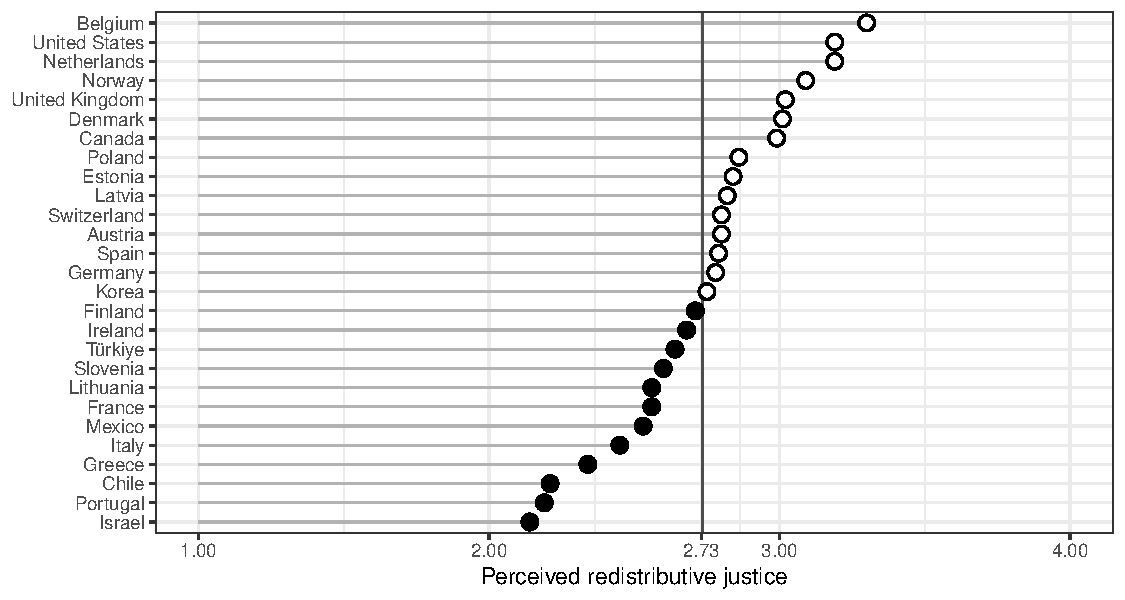
\includegraphics[width=0.85\linewidth,height=\textheight,keepaspectratio]{paper_files/figure-pdf/fig-cleveland-1.pdf}

}

\subcaption{\label{fig-cleveland}Source: own elaboration with data from
the OECD, Risks That Matter survey 2024. Perceived redistributive
justice corresponds to the degree of agreement with the item on
receiving a fair share of public benefits given the taxes and
contributions paid (scale 1--5). The vertical grey line shows the OECD
mean of redistributive justice.}

}

\end{figure}%

\subsection{Work, type of employment and platform
economy}\label{work-type-of-employment-and-platform-economy}

The sociology of work has documented in multiple contexts the growing
polarisation between formal, well-paid employment and an expanding
stratum of precarious work (\citeproc{ref-gallie_economic_2013}{Gallie,
2013}; \citeproc{ref-kalleberg_good_2011}{Kalleberg, 2011}). The concept
of precarious work, understood as uncertain and unpredictable employment
that shifts risk from employers to workers, describes a condition that
has spread beyond the margins of the labour market to reach growing
portions of the workforce (\citeproc{ref-kalleberg_good_2011}{Kalleberg,
2011}). Standing (\citeproc{ref-standing_precariat_2014}{2014}) 's
notion of precarity adds that this condition is not reduced to income
insecurity, but entails the absence of the occupational identity, social
rights and temporal stability that characterised the standard employment
relationship. These transformations matter for the welfare state because
its institutions were designed around that formal relationship, so that
those who depart from it tend to maintain a weaker and more unequal link
with the protection system
(\citeproc{ref-emmenegger_age_2012}{Emmenegger et al., 2012};
\citeproc{ref-schwander_who_2013}{Schwander and Häusermann, 2013}). This
structural position in the labour market shapes that material link, and
also conditions attitudes towards inequality and redistribution
(\citeproc{ref-lindh_class_2020}{Lindh and McCall, 2020}), an effect
especially visible in contexts of marked commodification such as the
Chilean one
(\citeproc{ref-perez-ahumada_conditioning_2026}{Pérez-Ahumada et al.,
2026}).

Type of employment structures that relationship directly. Workers in
formal waged employment contribute through registered contributions and
accumulate rights in a legible way, which makes the relationship between
what they contribute and what they receive traceable. Workers in
non-formal employment face a more opaque and often less favourable
relationship, since the self-employed tend to pay higher net
contributions and remain excluded from unemployment insurance, while
temporary workers accumulate interrupted contribution records that
reduce their future benefits (\citeproc{ref-marx_effect_2014}{Marx,
2014}; \citeproc{ref-rueda_social_2007}{Rueda, 2007}). This
institutional distance between insiders and outsiders in the labour
market creates conditions for the latter to perceive that the system was
not designed for people in their situation, which may translate into a
less favourable assessment of the fairness of the fiscal exchange
(\citeproc{ref-schwander_who_2013}{Schwander and Häusermann, 2013}).

Platform-mediated work constitutes a particularly acute form of
non-formal employment. Algorithmic intermediation, the classification of
workers as independent contractors and the fragmentation of tasks place
these workers largely outside the formal architecture of social
insurance (\citeproc{ref-vallas_what_2020}{Vallas and Schor, 2020};
\citeproc{ref-wood_good_2019}{Wood et al., 2019}). Several studies have
shown that platform workers combine nominal autonomy with a high degree
of external control and a fragmented or non-existent social protection
(\citeproc{ref-behrendt_social_2019}{Behrendt et al., 2019};
\citeproc{ref-schor_gig_2020}{Schor, 2020}), a pattern that evidence for
Latin America has documented in platform-mediated delivery, where
classification as independent contractors shifts risk onto workers and
leaves them outside social security
(\citeproc{ref-gutierrezcrocco_effects_2022}{Gutiérrez Crocco and
Atzeni, 2022}). This structural position exposes them to a lack of
protection that leads one to expect a comparatively lower perception of
the fairness of their relationship with the welfare state. These
considerations give rise to the first hypothesis:

\begin{tcolorbox}[enhanced jigsaw, arc=.35mm, bottomrule=.15mm, breakable, colback=white, colframe=quarto-callout-color-frame, left=2mm, leftrule=.75mm, opacityback=0, rightrule=.15mm, toprule=.15mm]

H1: Workers in non-formal employment ---platform work and
self-employment--- will perceive lower redistributive justice than
workers in formal waged employment.

\end{tcolorbox}

\subsection{Job insecurity}\label{job-insecurity}

Beyond type of employment, the level of job insecurity experienced by
workers constitutes a distinct dimension of vulnerability. Job
insecurity is defined as the subjective assessment of the likelihood of
losing one's own job or self-employment income in the short term, and
captures the chronic uncertainty and anticipatory anxiety associated
with the possibility of job loss (\citeproc{ref-dewitte_job_2005}{De
Witte, 2005}; \citeproc{ref-sverke_no_2002}{Sverke et al., 2002}).
Unlike objective precarity, it is a perceived state that can also affect
formally protected workers and whose effects on behaviour and attitudes
are widely documented (\citeproc{ref-anderson_workers_2007}{Anderson and
Pontusson, 2007}; \citeproc{ref-chung_institutions_2011}{Chung and Van
Oorschot, 2011}).

From the perspective of redistributive justice, job insecurity raises
what is at stake in the relationship between contributions and benefits.
The literature on risk and redistribution has shown that exposure to
insecurity increases support for social protection
(\citeproc{ref-cusack_risks_2006}{Cusack et al., 2006};
\citeproc{ref-iversen_asset_2001}{Iversen and Soskice, 2001};
\citeproc{ref-rehm_risks_2009}{Rehm, 2009}). The relationship with
perceived fairness may, however, operate in a different direction:
workers who anticipate losing their job assess with greater scrutiny
what they would receive from the state in that scenario, and when that
expectation is not accompanied by confidence in the protective capacity
of the system, they are likely to perceive the exchange as less fair
(\citeproc{ref-marx_effect_2014}{Marx, 2014}). The second hypothesis is
thus proposed:

\begin{tcolorbox}[enhanced jigsaw, arc=.35mm, bottomrule=.15mm, breakable, colback=white, colframe=quarto-callout-color-frame, left=2mm, leftrule=.75mm, opacityback=0, rightrule=.15mm, toprule=.15mm]

H2: Greater perceived job insecurity will be associated with a lower
perception of redistributive justice.

\end{tcolorbox}

\subsection{Perceived technological
change}\label{perceived-technological-change}

The rise of digital technologies has introduced an additional source of
occupational vulnerability, distinct from conventional job insecurity.
Estimates of the proportion of jobs susceptible to automation vary
widely, but even the most conservative ones anticipate significant
changes in the content of tasks and in the viability of numerous
occupations (\citeproc{ref-arntz_risk_2016}{Arntz et al., 2016};
\citeproc{ref-autor_why_2015}{Autor, 2015};
\citeproc{ref-bustelo_automation_2020}{Bustelo et al., 2020};
\citeproc{ref-frey_future_2017}{Frey and Osborne, 2017}). What matters
for welfare attitudes is not the objective magnitude of that process,
but the way in which workers anticipate its effects on their own job
(\citeproc{ref-gallego_automation_2022}{Gallego and Kurer, 2022}). That
anticipation comprises both the perception of a displacement risk (the
probability of losing the job to technology) and the perception of a
benefit (the probability that technology will improve the quality of
work).

\subsubsection{Perception of technological displacement
risk}\label{perception-of-technological-displacement-risk}

On the one hand, technological change refers to the perception of
technological displacement risk, that is, the probability that one's own
job will be replaced by a robot or by artificial intelligence,
substituted by a provider offering a similar service through a platform,
or rendered unviable by the obsolescence of one's own digital skills.
Research has shown that the fear of automation is distributed unevenly
across occupations and social groups and that it has measurable
political and attitudinal consequences
(\citeproc{ref-dekker_fear_2017}{Dekker et al., 2017};
\citeproc{ref-im_losers_2019}{Im et al., 2019};
\citeproc{ref-kurer_declining_2020}{Kurer, 2020}). Within the framework
of welfare attitudes, the literature on risk and redistribution has
robustly established that perceived exposure to technological risk
increases the demand for social protection and is associated with an
experience of economic insecurity
(\citeproc{ref-busemeyer_social_2022}{Busemeyer and Sahm, 2022};
\citeproc{ref-iversen_asset_2001}{Iversen and Soskice, 2001};
\citeproc{ref-rehm_risks_2009}{Rehm, 2009};
\citeproc{ref-thewissen_automation_2019}{Thewissen and Rueda, 2019}).
Following that logic, workers who perceive their job as threatened by
technology hold greater expectations of protection and, when contrasting
these with what they actually receive, are more likely to assess their
exchange with the welfare state as insufficient
(\citeproc{ref-marx_effect_2014}{Marx, 2014}). The third hypothesis is
thus derived:

\begin{tcolorbox}[enhanced jigsaw, arc=.35mm, bottomrule=.15mm, breakable, colback=white, colframe=quarto-callout-color-frame, left=2mm, leftrule=.75mm, opacityback=0, rightrule=.15mm, toprule=.15mm]

H3: Workers who perceive a higher probability of being displaced by
automation, platform competition or the obsolescence of their skills
will report a lower perception of distributive justice.

\end{tcolorbox}

\subsubsection{Perception of technological
benefit}\label{perception-of-technological-benefit}

On the other hand, technological change refers to the perception of
technological benefit, which addresses the probability that technology
will make working hours more compatible with private life, reduce the
dangerousness or physical demands of work, or lessen its monotony and
mental load. This enabling dimension has received much less attention
than its threatening counterpart, even though workers' orientation
towards technology is not solely negative
(\citeproc{ref-autor_why_2015}{Autor, 2015};
\citeproc{ref-brougham_smart_2018}{Brougham and Haar, 2018}). Unlike
displacement risk, perceiving technology as an improvement in working
conditions places the worker in a position of lower exposure to risk and
greater optimism about their occupational trajectory. To the extent that
the assessment of the exchange with the welfare state reflects the
individual's position of economic security
(\citeproc{ref-rehm_risks_2009}{Rehm, 2009}), this positive orientation
can be expected to be associated with a more favourable perception of
redistributive justice. The fourth hypothesis follows from this:

\begin{tcolorbox}[enhanced jigsaw, arc=.35mm, bottomrule=.15mm, breakable, colback=white, colframe=quarto-callout-color-frame, left=2mm, leftrule=.75mm, opacityback=0, rightrule=.15mm, toprule=.15mm]

H4: Workers who perceive technology as enabling ---reducing physical
demands, improving the balance between work and private life or making
work less stressful or monotonous--- will perceive greater
redistributive justice.

\end{tcolorbox}

\subsection{Perceived deservingness of
others}\label{perceived-deservingness-of-others}

Perceptions of redistributive justice do not depend solely on structural
position, but also on the normative frameworks through which individuals
assess who and what deserves to receive from the state. Deservingness
theory holds that people direct their solidarity towards the groups they
consider deserving and withdraw it from those they judge undeserving, on
the basis of criteria such as control over one's own situation,
attitude, reciprocity, identity and need
(\citeproc{ref-petersen_social_2012}{Petersen, 2012};
\citeproc{ref-oorschot_who_2000}{Van Oorschot, 2000}). In strongly
commodified contexts, meritocratic and market-justice beliefs reinforce
the tendency to assess the recipients of state support in terms of merit
and, with it, to consider undeserving those who are perceived not to
contribute enough (\citeproc{ref-castillo_perceptions_2025}{Castillo et
al., 2025}). These judgements about the deservingness of others are
analytically distinct from the judgement that each individual makes
about the fairness of their own relationship with the system. The
distinction is relevant, since a person may consider themselves a
contributor who does not receive their fair share and, at the same time,
judge that others receive benefits they do not deserve. Both assessments
are, however, part of the same moral economy of welfare, and they can be
expected to be connected (\citeproc{ref-mau_moral_2014}{Mau, 2014};
\citeproc{ref-vanoorschot_social_2017}{Van Oorschot et al., 2017}).

The connection between the two judgements operates through the norm of
reciprocity. The resources that an individual contributes appear to
sustain those who do not fulfil their part, which erodes the sense that
the system treats them fairly
(\citeproc{ref-cavaille_fair_2025}{Cavaillé, 2025};
\citeproc{ref-reeskens_equity_2013}{Reeskens and Van Oorschot, 2013}).
Comparative research has shown that deservingness perceptions robustly
structure support for the welfare state and that the control criterion
occupies a central place in those judgements
(\citeproc{ref-laenen_welfare_2020}{Laenen, 2020};
\citeproc{ref-vanoorschot_making_2006}{Van Oorschot, 2006}). It can
therefore be expected that those who perceive greater abuse of the
system by others will assess their own relationship with it as less
fair. The fifth hypothesis is proposed:

\begin{tcolorbox}[enhanced jigsaw, arc=.35mm, bottomrule=.15mm, breakable, colback=white, colframe=quarto-callout-color-frame, left=2mm, leftrule=.75mm, opacityback=0, rightrule=.15mm, toprule=.15mm]

H5: Workers who perceive that many people receive public benefits
without deserving them will report a lower perception of redistributive
justice.

\end{tcolorbox}

\subsection{Welfare regimes and institutional
context}\label{welfare-regimes-and-institutional-context}

Individual perceptions of redistributive justice are formed in
institutional contexts that vary systematically across welfare regimes
(\citeproc{ref-arts_three_2002}{Arts and Gelissen, 2002};
\citeproc{ref-esping-andersen_three_1993}{Esping-Andersen, 1993}).
Esping-Andersen (\citeproc{ref-esping-andersen_three_1993}{1993}) 's
classic typology distinguishes three worlds of welfare capitalism
according to how they organise the relationship between state, market
and family in the provision of social protection. In social democratic
regimes (mainly Nordic countries), protection is comprehensive and
universal, and redistribution constitutes a central expression of social
solidarity sustained by universalist institutions
(\citeproc{ref-korpi_paradox_1998}{Korpi and Palme, 1998}). In liberal
regimes (mainly Anglo-Saxon countries and, for example, Chile as a case
of a commodified welfare state in Latin America), protection is residual
and targeted, is organised around market participation and is
politically more contested Pérez-Ahuamda
(\citeproc{ref-perez_building_2023}{2023}). In conservative-corporatist
regimes (continental Europe), rights are strongly tied to employment
status, which preserves status differences and links protection to the
employment trajectory (\citeproc{ref-ferrera_southern_1996}{Ferrera,
1996}).

Alongside institutional design, macroeconomic factors such as the level
of income per capita and the degree of inequality bear on welfare
attitudes. The evidence suggests that income inequality is associated
with perceptions of the fairness of the system, although the direction
of that relationship is a matter of debate
(\citeproc{ref-finseraas_income_2009}{Finseraas, 2009};
\citeproc{ref-schmidt-catran_economic_2016}{Schmidt-Catran, 2016}), and
that the level of economic development conditions both the fiscal
capacity of the state and citizens' expectations regarding social
protection (\citeproc{ref-blekesaune_public_2003}{Blekesaune, 2003}).
Taken together, the perception of redistributive justice can be expected
to be, on average, higher in social democratic regimes, where protection
is more comprehensive and universal, than in liberal and conservative
regimes (\citeproc{ref-jaeger_welfare_2006}{Jæger, 2006};
\citeproc{ref-larsen_institutional_2008}{Larsen, 2008};
\citeproc{ref-svallfors_worlds_1997}{Svallfors, 1997}). Hence the sixth
hypothesis:

\begin{tcolorbox}[enhanced jigsaw, arc=.35mm, bottomrule=.15mm, breakable, colback=white, colframe=quarto-callout-color-frame, left=2mm, leftrule=.75mm, opacityback=0, rightrule=.15mm, toprule=.15mm]

H6: On average, workers in social democratic regimes will perceive
higher redistributive justice than workers in liberal and conservative
regimes.

\end{tcolorbox}

The institutional context not only shifts the average level of
perceptions, but may moderate the effect of individual predictors. The
institutional distance between workers in non-formal employment and the
protection system is greater in liberal and conservative regimes than in
social democratic ones, which are universalist in character
(\citeproc{ref-ferrera_southern_1996}{Ferrera, 1996};
\citeproc{ref-schwander_who_2013}{Schwander and Häusermann, 2013}). It
can therefore be expected that the negative effect of labour market
position on perceived fairness will be more pronounced in the former:

\begin{tcolorbox}[enhanced jigsaw, arc=.35mm, bottomrule=.15mm, breakable, colback=white, colframe=quarto-callout-color-frame, left=2mm, leftrule=.75mm, opacityback=0, rightrule=.15mm, toprule=.15mm]

H7: The negative relationship between non-standard employment (platform
work and self-employment) and perceived redistributive justice will be
moderated by the welfare regime.

\end{tcolorbox}

An analogous expectation can be formulated for the perception of
technological risk. In universalist regimes, protection against the
risks associated with digitalisation is more robust and less dependent
on the individual employment trajectory, which could cushion the effect
of perceived displacement risk on the assessment of the fiscal exchange
(\citeproc{ref-busemeyer_social_2022}{Busemeyer and Sahm, 2022};
\citeproc{ref-fan_how_2024}{Fan et al., 2024};
\citeproc{ref-gallego_automation_2022}{Gallego and Kurer, 2022}):

\begin{tcolorbox}[enhanced jigsaw, arc=.35mm, bottomrule=.15mm, breakable, colback=white, colframe=quarto-callout-color-frame, left=2mm, leftrule=.75mm, opacityback=0, rightrule=.15mm, toprule=.15mm]

H8: The negative effect of the perception of technological displacement
risk on the perception of redistributive justice will be moderated by
the welfare regime.

\end{tcolorbox}

Finally, the salience of deservingness judgements varies according to
institutional design. In universalist regimes, where benefits are
conceived as general rights rather than as targeted assistance, the
distinctions between deserving and undeserving tend to be less
pronounced than in residual regimes, organised around means testing
(\citeproc{ref-larsen_institutional_2008}{Larsen, 2008};
\citeproc{ref-vanoorschot_social_2017}{Van Oorschot et al., 2017}). It
can therefore be expected that the effect of the perceived deservingness
of others on the fairness of one's own exchange will be stronger in
liberal and conservative regimes:

\begin{tcolorbox}[enhanced jigsaw, arc=.35mm, bottomrule=.15mm, breakable, colback=white, colframe=quarto-callout-color-frame, left=2mm, leftrule=.75mm, opacityback=0, rightrule=.15mm, toprule=.15mm]

H9: The negative effect of the perceived deservingness of others on the
perception of redistributive justice will be moderated by the welfare
regime.

\end{tcolorbox}

\section{Data, variables and methods}\label{data-variables-and-methods}

\subsection{Data}\label{data}

This study uses data from the Risks That Matter (RTM) survey of the
OECD, a cross-national public opinion survey applied in 27 member
countries of the Organisation for Economic Co-operation and Development.
The most recent wave (2024) is used, which includes more than 40,000
people across 27 OECD countries: Australia, Austria, Belgium, Canada,
Chile, Colombia, Costa Rica, the Czech Republic, Denmark, Estonia,
Finland, France, Germany, Greece, Hungary, Ireland, Israel, Italy,
Japan, Korea, Lithuania, Mexico, the Netherlands, New Zealand, Poland,
Portugal and the United States. The survey collects nationally
representative data on adults aged between 18 and 64, using stratified
sampling with post-stratification weights calibrated by age, sex, region
and educational level. The 2024 wave is especially relevant for this
study because it captures attitudes in the period following the COVID-19
pandemic, an episode that dramatically accelerated the digitalisation of
work, expanded platform employment and exposed the cracks in the social
insurance systems of the OECD countries.

\subsection{Variables}\label{variables}

The dependent variable is the perception of redistributive justice,
measured by the item: ``I feel that I receive a fair share of public
benefits, given the taxes and social contributions that I pay and/or
have paid in the past'', answered on a five-point Likert scale ranging
from strongly disagree to strongly agree. This item captures the
person's evaluative judgement of the fairness of the exchange with the
state and is treated as an ordinal variable in all the analyses.

Three sets of independent variables constitute the core of the analysis.
The first concerns labour market position and job insecurity. Type of
employment is operationalised as a three-category variable
distinguishing formal waged employment (permanent or long-term dependent
employment), platform work (work mediated by digital platforms) and
self-employment. Job insecurity is measured by the item: ``How likely do
you think it is that you could lose your job or your self-employment
income in the next 12 months?'', with response categories ranging from
very unlikely to very likely. This item captures the subjective,
anticipatory dimension of precarity: workers' sense of how exposed they
are to income loss in the short term.

The second set of variables captures the perception of technological
change with respect to one's own job. These variables are measured
through a battery that asks: ``How likely do you think it is that the
following will happen in your job (or job opportunities) in the next
five years?'', with items rated on a four-point probability scale. The
battery includes four displacement items ---the likelihood that the job
will be replaced by a robot, that it will be replaced by an artificial
intelligence tool such as ChatGPT, and that it will be replaced by a
person offering a similar service through an internet platform, and the
likelihood of losing the job through not being sufficiently
technologically skilled--- and three benefit items ---that technology
will make working hours more compatible with private life, that it will
make work less dangerous or physically demanding, and that it will make
it less boring, repetitive, stressful or mentally demanding. However,
the exploratory factor analysis carried out on these seven items yields
a three-factor structure: the three displacement items load on a first
factor; the three benefit items load on a second factor; and the skill
obsolescence item separates from both, so that it is retained as a
single indicator, capturing an internal element of risk perception,
distinct from the other two factors, which are considered external
elements. Following the usual practice in constructing composite indices
from attitudinal batteries, two scales are built ---Technological
Displacement Risk (the average of the three displacement items) and
Perceived Technological Benefit (the average of the three benefit
items)--- and Perceived Skill Obsolescence is used as a single item. In
all cases, higher values indicate a greater perception of the
corresponding risk or benefit.

The third set of independent variables concerns the perceived
deservingness of others, operationalised through the item that measures
the degree of agreement with the statement «Many people receive public
benefits without deserving them», rated on a five-point scale (1 =
strongly disagree to 5 = strongly agree). Unlike the dependent variable,
which captures the individual's judgement of the fairness of their own
relationship with the system, this item captures their judgement of the
deservingness of other beneficiaries, a central distinction in the
literature on deservingness (\citeproc{ref-vanoorschot_making_2006}{Van
Oorschot, 2006}, \citeproc{ref-oorschot_who_2000}{2000}). Higher values
indicate a more widespread perception of undue deservingness on the part
of third parties.

The welfare regime is operationalised as a three-category variable
(social democratic, liberal, conservative-corporatist) following Bambra
(\citeproc{ref-bambra_sifting_2007}{2007}) and Fenger
(\citeproc{ref-Fenger2006WelfareRI}{2006}). To classify the countries of
southern Europe and of central and eastern Europe present in the sample,
the extensions of Ferrera (\citeproc{ref-ferrera_southern_1996}{1996}),
Fenger (\citeproc{ref-Fenger2006WelfareRI}{2006}) and Aidukaite
(\citeproc{ref-aidukaite_welfare_2011}{2011}) are followed, which
document both the initial specificity of the post-socialist regimes and
their progressive convergence towards the continental types after two
decades of transition. On that basis, and given the small number of
countries per category, the study adopts a three-regime classification
---social democratic, liberal and conservative-corporatist---, in which
the countries of southern Europe and of central and eastern Europe are
integrated into the conservative category, while the Baltic states,
characterised by a more liberal orientation of their post-socialist
reforms, are incorporated into the liberal regime
(\citeproc{ref-aidukaite_welfare_2011}{Aidukaite, 2011}).

All the models include a set of control variables that have been shown
to be associated with attitudes towards the welfare state and perceived
redistributive justice: sex, age, educational level (operationalised as
the highest level of studies completed) and income decile (self-reported
position in the national income distribution).

A summary of these variables and their main descriptive statistics is
available in Table~\ref{tbl-summary}

\begin{longtable}[]{@{}
  >{\raggedright\arraybackslash}p{(\linewidth - 6\tabcolsep) * \real{0.3925}}
  >{\raggedright\arraybackslash}p{(\linewidth - 6\tabcolsep) * \real{0.3084}}
  >{\raggedright\arraybackslash}p{(\linewidth - 6\tabcolsep) * \real{0.1963}}
  >{\raggedright\arraybackslash}p{(\linewidth - 6\tabcolsep) * \real{0.1028}}@{}}
\caption{Main descriptive statistics}\label{tbl-summary}\tabularnewline
\toprule\noalign{}
\begin{minipage}[b]{\linewidth}\raggedright
Label
\end{minipage} & \begin{minipage}[b]{\linewidth}\raggedright
Stats / Values
\end{minipage} & \begin{minipage}[b]{\linewidth}\raggedright
Freqs (\% of Valid)
\end{minipage} & \begin{minipage}[b]{\linewidth}\raggedright
Valid
\end{minipage} \\
\midrule\noalign{}
\endfirsthead
\toprule\noalign{}
\begin{minipage}[b]{\linewidth}\raggedright
Label
\end{minipage} & \begin{minipage}[b]{\linewidth}\raggedright
Stats / Values
\end{minipage} & \begin{minipage}[b]{\linewidth}\raggedright
Freqs (\% of Valid)
\end{minipage} & \begin{minipage}[b]{\linewidth}\raggedright
Valid
\end{minipage} \\
\midrule\noalign{}
\endhead
\bottomrule\noalign{}
\endlastfoot
Redistributive justice & \begin{minipage}[t]{\linewidth}\raggedright
1. Strongly disagree\\
2. Disagree\\
3. Neither agree nor disagre\\
4. Agree\\
5. Strongly agree\strut
\end{minipage} & \begin{minipage}[t]{\linewidth}\raggedright
3506 (18.3\%)\\
4651 (24.3\%)\\
5466 (28.5\%)\\
4162 (21.7\%)\\
1384 ( 7.2\%)\strut
\end{minipage} & \begin{minipage}[t]{\linewidth}\raggedright
19169\\
(100.0\%)\strut
\end{minipage} \\
Sex & \begin{minipage}[t]{\linewidth}\raggedright
1. Man\\
2. Woman\strut
\end{minipage} & \begin{minipage}[t]{\linewidth}\raggedright
10293 (53.7\%)\\
8876 (46.3\%)\strut
\end{minipage} & \begin{minipage}[t]{\linewidth}\raggedright
19169\\
(100.0\%)\strut
\end{minipage} \\
Age group & \begin{minipage}[t]{\linewidth}\raggedright
1. 18-24\\
2. 25-34\\
3. 35-44\\
4. 45-54\\
5. 55-64\strut
\end{minipage} & \begin{minipage}[t]{\linewidth}\raggedright
2076 (10.8\%)\\
4522 (23.6\%)\\
4726 (24.7\%)\\
4486 (23.4\%)\\
3359 (17.5\%)\strut
\end{minipage} & \begin{minipage}[t]{\linewidth}\raggedright
19169\\
(100.0\%)\strut
\end{minipage} \\
Educational level & \begin{minipage}[t]{\linewidth}\raggedright
1. Low\\
2. Medium\\
3. High\strut
\end{minipage} & \begin{minipage}[t]{\linewidth}\raggedright
1494 ( 7.8\%)\\
7913 (41.3\%)\\
9762 (50.9\%)\strut
\end{minipage} & \begin{minipage}[t]{\linewidth}\raggedright
19169\\
(100.0\%)\strut
\end{minipage} \\
Equivalised disposable household income decile (2023) &
\begin{minipage}[t]{\linewidth}\raggedright
Mean (sd) : 4.9 (2.9)\\
min \textless{} med \textless{} max:\\
1 \textless{} 5 \textless{} 10\\
IQR (CV) : 5 (0.6)\strut
\end{minipage} & \begin{minipage}[t]{\linewidth}\raggedright
1 : 3288 (17.2\%)\\
2 : 1797 ( 9.4\%)\\
3 : 1723 ( 9.0\%)\\
4 : 2587 (13.5\%)\\
5 : 2273 (11.9\%)\\
6 : 1777 ( 9.3\%)\\
7 : 1447 ( 7.5\%)\\
8 : 1401 ( 7.3\%)\\
9 : 1272 ( 6.6\%)\\
10 : 1604 ( 8.4\%)\strut
\end{minipage} & \begin{minipage}[t]{\linewidth}\raggedright
19169\\
(100.0\%)\strut
\end{minipage} \\
Self-empleoyment worker & \begin{minipage}[t]{\linewidth}\raggedright
1. No\\
2. Yes\strut
\end{minipage} & \begin{minipage}[t]{\linewidth}\raggedright
16459 (85.9\%)\\
2710 (14.1\%)\strut
\end{minipage} & \begin{minipage}[t]{\linewidth}\raggedright
19169\\
(100.0\%)\strut
\end{minipage} \\
Platform worker & \begin{minipage}[t]{\linewidth}\raggedright
1. No\\
2. Yes\strut
\end{minipage} & \begin{minipage}[t]{\linewidth}\raggedright
17361 (90.6\%)\\
1808 ( 9.4\%)\strut
\end{minipage} & \begin{minipage}[t]{\linewidth}\raggedright
19169\\
(100.0\%)\strut
\end{minipage} \\
Lose job & \begin{minipage}[t]{\linewidth}\raggedright
1. Not at all concerned\\
2. Not so concerned\\
3. Somewhat concerned\\
4. Very concerned\strut
\end{minipage} & \begin{minipage}[t]{\linewidth}\raggedright
2867 (15.0\%)\\
5351 (27.9\%)\\
5920 (30.9\%)\\
5031 (26.2\%)\strut
\end{minipage} & \begin{minipage}[t]{\linewidth}\raggedright
19169\\
(100.0\%)\strut
\end{minipage} \\
Technological displacement & \begin{minipage}[t]{\linewidth}\raggedright
Mean (sd) : 2.1 (0.9)\\
min \textless{} med \textless{} max:\\
1 \textless{} 2 \textless{} 4\\
IQR (CV) : 1.7 (0.4)\strut
\end{minipage} & 13 distinct values &
\begin{minipage}[t]{\linewidth}\raggedright
19169\\
(100.0\%)\strut
\end{minipage} \\
Perceived technological benefit &
\begin{minipage}[t]{\linewidth}\raggedright
Mean (sd) : 2.6 (0.8)\\
min \textless{} med \textless{} max:\\
1 \textless{} 2.7 \textless{} 4\\
IQR (CV) : 1 (0.3)\strut
\end{minipage} & 13 distinct values &
\begin{minipage}[t]{\linewidth}\raggedright
19169\\
(100.0\%)\strut
\end{minipage} \\
Lose job due skills & \begin{minipage}[t]{\linewidth}\raggedright
1. Very unlikely\\
2. Unlikely\\
3. Likely\\
4. Very likely\strut
\end{minipage} & \begin{minipage}[t]{\linewidth}\raggedright
6218 (32.4\%)\\
6595 (34.4\%)\\
4546 (23.7\%)\\
1810 ( 9.4\%)\strut
\end{minipage} & \begin{minipage}[t]{\linewidth}\raggedright
19169\\
(100.0\%)\strut
\end{minipage} \\
Deservingness of others & \begin{minipage}[t]{\linewidth}\raggedright
1. Strongly disagree\\
2. Disagree\\
3. Neither agree nor disagre\\
4. Agree\\
5. Strongly agree\strut
\end{minipage} & \begin{minipage}[t]{\linewidth}\raggedright
611 ( 3.2\%)\\
1683 ( 8.8\%)\\
4299 (22.4\%)\\
6504 (33.9\%)\\
6072 (31.7\%)\strut
\end{minipage} & \begin{minipage}[t]{\linewidth}\raggedright
19169\\
(100.0\%)\strut
\end{minipage} \\
GDP per-capita & \begin{minipage}[t]{\linewidth}\raggedright
Mean (sd) : 49908.9 (26346.1)\\
min \textless{} med \textless{} max:\\
13826 \textless{} 46150 \textless{} 112356\\
IQR (CV) : 28994 (0.5)\strut
\end{minipage} & 27 distinct values &
\begin{minipage}[t]{\linewidth}\raggedright
19169\\
(100.0\%)\strut
\end{minipage} \\
Welfare regime & \begin{minipage}[t]{\linewidth}\raggedright
1. Liberal\\
2. Social-democratic\\
3. Conservative\strut
\end{minipage} & \begin{minipage}[t]{\linewidth}\raggedright
6397 (33.4\%)\\
2888 (15.1\%)\\
9884 (51.6\%)\strut
\end{minipage} & \begin{minipage}[t]{\linewidth}\raggedright
19169\\
(100.0\%)\strut
\end{minipage} \\
\end{longtable}

\subsection{Methods}\label{methods}

Multilevel ordinal logistic regression models with individuals nested in
countries are used to examine the relationship between labour market
position, the perception of technological risk or benefit, the
deservingness of others and the perception of redistributive justice
across different national contexts. This approach makes it possible to
account for the hierarchical structure of the comparative data and to
decompose the variance of the outcome between individual factors and
country characteristics (\citeproc{ref-hox_multilevel_2017}{Hox et al.,
2017}; \citeproc{ref-snijders_multilevel_2012}{Snijders and Bosker,
2012}). Random intercepts are estimated for each country to control
heterogeneity at the macro level. The models are estimated sequentially:
a model including if the workers are self-employed or platform-worker
(Model 1), a second model adding job insecurity (Model 2), a third model
incorporating the perception of technological risk and benefit (Model
3), a fourth model adding the perception of the deservingness of others
(Model 4), a fifth model incorporating the type of welfare regime (Model
5), and a sixt model adding the control variables (Model 6).

In a seven model, interaction terms between the labour market predictors
are introduced (Model 7). In the next models, the type of welfare regime
are introduced to test the rest of moderation hypotheses (Models 8 to
models 12). All the analyses use the individual survey weights provided
by the OECD, and standard errors are clustered by country. The models
are estimated with the clmm function of the ordinal package in R.

\section{Analysis}\label{analysis}



Figure~\ref{fig-correlation} presents a correlation matrix of the main
variables analyzed. In this matrix, the correlations vary between low
and moderate negative and positive values. The main correlation effects
are between perceived redistributive justice and being a platform worker
(r=0,32, p\textless0.001), the perceived technological displacement
(r=0,24, p\textless0,001), the skill obsolescence risk (r=0,26,
p\textless0,001), and the perceived technological benefit (r=0,21,
p\textless0,001) which are positive and moderated effects. In other
sence, the deservingess of others has a negative and moderated effect
(r=0,16, p\textless0,01).

Regarding the independent variables, the main correlation effects are
between the corcern about job and income loss and being a platform
worker (r=0,15, p\textless0,001), and with the perceived of
technological change variables. Between this this three last variables,
the correlations effects are positive and significant, contrary to the
initial intuitions.

\begin{figure}[H]

\caption{\label{fig-correlation}Correlation matrix of the main
variables}

\centering{

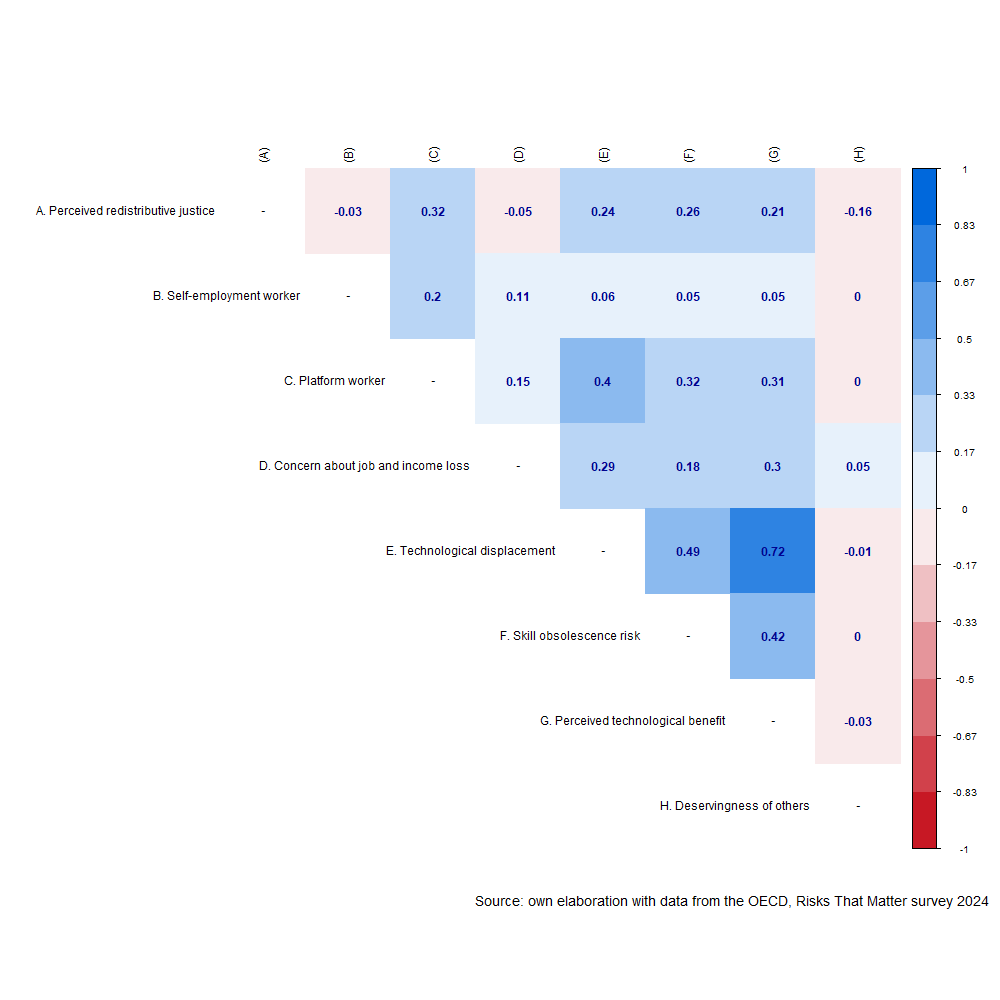
\includegraphics[width=0.85\linewidth,height=\textheight,keepaspectratio]{output/figures/corrplot.png}

}

\end{figure}%

\subsection{Multilevel ordinal logistic regression
models}\label{multilevel-ordinal-logistic-regression-models}

\begin{Shaded}
\begin{Highlighting}[]
\CommentTok{\# DV como factor}
\FunctionTok{sum}\NormalTok{(}\FunctionTok{is.na}\NormalTok{(data}\SpecialCharTok{$}\NormalTok{distributive))}
\end{Highlighting}
\end{Shaded}

\begin{verbatim}
[1] 0
\end{verbatim}

\begin{Shaded}
\begin{Highlighting}[]
\FunctionTok{table}\NormalTok{(data}\SpecialCharTok{$}\NormalTok{distributive, }\AttributeTok{useNA =} \StringTok{"ifany"}\NormalTok{)}
\end{Highlighting}
\end{Shaded}

\begin{verbatim}

   1    2    3    4    5 
3506 4651 5466 4162 1384 
\end{verbatim}

\begin{Shaded}
\begin{Highlighting}[]
\CommentTok{\# Conversión numérica: ¿mismos NA?}
\FunctionTok{sum}\NormalTok{(}\FunctionTok{is.na}\NormalTok{(}\FunctionTok{as.numeric}\NormalTok{(data}\SpecialCharTok{$}\NormalTok{distributive)))}
\end{Highlighting}
\end{Shaded}

\begin{verbatim}
[1] 0
\end{verbatim}

\begin{Shaded}
\begin{Highlighting}[]
\FunctionTok{table}\NormalTok{(}\FunctionTok{as.numeric}\NormalTok{(data}\SpecialCharTok{$}\NormalTok{distributive), }\AttributeTok{useNA =} \StringTok{"ifany"}\NormalTok{)}
\end{Highlighting}
\end{Shaded}

\begin{verbatim}

   1    2    3    4    5 
3506 4651 5466 4162 1384 
\end{verbatim}

\begin{Shaded}
\begin{Highlighting}[]
\CommentTok{\# Peso: ¿NA o ceros?}
\FunctionTok{sum}\NormalTok{(}\FunctionTok{is.na}\NormalTok{(data}\SpecialCharTok{$}\NormalTok{weight)); }\FunctionTok{sum}\NormalTok{(data}\SpecialCharTok{$}\NormalTok{weight }\SpecialCharTok{==} \DecValTok{0}\NormalTok{, }\AttributeTok{na.rm =} \ConstantTok{TRUE}\NormalTok{)}
\end{Highlighting}
\end{Shaded}

\begin{verbatim}
[1] 0
\end{verbatim}

\begin{verbatim}
[1] 0
\end{verbatim}

\begin{Shaded}
\begin{Highlighting}[]
\FunctionTok{summary}\NormalTok{(data}\SpecialCharTok{$}\NormalTok{weight)}
\end{Highlighting}
\end{Shaded}

\begin{verbatim}
   Min. 1st Qu.  Median    Mean 3rd Qu.    Max. 
 0.1219  0.5931  0.7869  0.8802  1.0547  8.2564 
\end{verbatim}

\begin{table}

\caption{\label{tbl-modelos}Multilevel models for retributive
preferences}

\centering{

~

Model 1

Model 2

Model 3

Model 4

Model 5

Model 6

self-employed worker (ref. No)

-0.059

-0.057

-0.057

-0.068

-0.068

-0.069

~

(0.039)

(0.039)

(0.039)

(0.039)

(0.039)

(0.039)

Platform worker (ref. No)

1.174***

1.189***

0.828***

0.844***

0.843***

0.780***

~

(0.050)

(0.050)

(0.051)

(0.051)

(0.051)

(0.051)

Concern about job and income loss

~

-0.054***

-0.180***

-0.175***

-0.176***

-0.166***

~

~

(0.014)

(0.015)

(0.015)

(0.015)

(0.015)

Technological displacement

~

~

0.265***

0.261***

0.261***

0.237***

~

~

~

(0.023)

(0.023)

(0.023)

(0.024)

Skill obsolescence risk

~

~

0.126***

0.123***

0.123***

0.126***

~

~

~

(0.020)

(0.020)

(0.020)

(0.020)

Perceived technological benefit

~

~

0.453***

0.456***

0.456***

0.431***

~

~

~

(0.021)

(0.021)

(0.021)

(0.022)

Deservingness of others

~

~

~

-0.181***

-0.181***

-0.177***

~

~

~

~

(0.014)

(0.014)

(0.014)

Welfare regime (Ref.= Liberal)

~

~

~

~

~

~

~

~

~

~

~

~

~

~~~~~Social-democratic

~

~

~

~

0.408

0.395

~

~

~

~

~

(0.267)

(0.267)

~~~~~Conservative

~

~

~

~

-0.138

-0.126

~

~

~

~

~

(0.190)

(0.190)

BIC

50264.921

50260.479

48843.271

48682.213

48697.344

48616.180

Numb. obs.

16872

16872

16872

16872

16872

16872

Groups (Country)

27

27

27

27

27

27

Variance: Country: (Intercept)

0.235

0.227

0.244

0.227

0.192

0.193

Note: Cells contain regression coefficients with standard errors in
parentheses. ***p \textless{} 0.001; **p \textless{} 0.01; *p
\textless{} 0.05. Model 6 is controlled by sex, age and income with
significant effects and education with no significant effect

}

\end{table}%

Cumulative-link mixed models were fitted for perceived redistributive
justice, with a random intercept for country. Note that ordinal package
reports the number of observations as the sum of the sampling weights
rather than the count of cases
(\citeproc{ref-haubo_cumulative_2018}{Haubo and Christensen, 2018}); the
models were therefore estimated on 19,169 respondents nested in 27
countries (weighted N = 16,872). Coefficients are cumulative log-odds: a
positive value indicates greater odds of reporting a higher category of
perceived redistributive justice.

Table~\ref{tbl-modelos} follows a block-building logic --- employment
status (Model 1), economic insecurity (Model 2), the
technological-perception battery (Model 3), deservingness of others
(Model 4) and welfare regime (Model 5) --- with sociodemographic
controls (sex, age, income and education) entered only in Model 6.
Across the sequence the country-level variance declines from 0.235 to
0.193 and the BIC from 50,264.9 to 48,616.2, indicating improved fit as
substantive predictors are added.

Platform work is the strongest and most stable predictor. In Model 1 its
coefficient is 1.174 (p \textless{} 0.001; OR ≈ 3.2); it attenuates as
the technological and deservingness blocks enter but remains large in
the fully adjusted Model 6 (0.780, p \textless{} 0.001; OR ≈ 2.2), so
platform workers have roughly twice the odds of expressing higher
perceived redistributive justice. Self-employment is non-significant
throughout (≈ −0.06). Concern about job and income loss is negative and
strengthens once technological perceptions are held constant, moving
from −0.054 in Model 2 to −0.166 in Model 6 (p \textless{} 0.001).

The technological-perception battery (from Model 3) is uniformly
positive. Perceived technological benefit carries the largest effect (≈
0.43--0.46, p \textless{} 0.001), followed by technological displacement
(≈ 0.24--0.27, p \textless{} 0.001) and skill-obsolescence risk (≈ 0.12,
p \textless{} 0.001). The positive sign on technological displacement
runs counter to the hypothesised direction, a point developed further in
the discussion. Deservingness of others (Model 4) is negative and stable
(≈ −0.18, p \textless{} 0.001). Welfare regime, entered as a main effect
in Model 5, is not significant: relative to liberal regimes, neither the
social-democratic (≈ 0.40) nor the conservative (≈ −0.13) contrast
reaches conventional thresholds. The addition of controls in Model 6
leaves this individual-level structure essentially unchanged.

\begin{table}

\caption{\label{tbl-interact}Interaction multilevel models for
retributive preferences}

\centering{

~

Model 1

Model 2

Model 3

Model 4

Model 5

Model 6

Self-employed worker (ref. No)

-0.018

0.009

-0.071

-0.068

-0.071

-0.071

~

(0.042)

(0.069)

(0.039)

(0.039)

(0.039)

(0.039)

Platform worker (ref. No)

0.877***

0.781***

0.953***

0.775***

0.777***

0.779***

~

(0.058)

(0.051)

(0.079)

(0.051)

(0.051)

(0.051)

Concern about job and income loss

-0.167***

-0.166***

-0.165***

-0.098***

-0.165***

-0.165***

~

(0.015)

(0.015)

(0.015)

(0.025)

(0.015)

(0.015)

Technological displacement

0.237***

0.238***

0.236***

0.238***

0.338***

0.236***

~

(0.024)

(0.024)

(0.024)

(0.024)

(0.032)

(0.024)

Deservingness of others

-0.176***

-0.177***

-0.177***

-0.177***

-0.178***

-0.122***

~

(0.014)

(0.014)

(0.014)

(0.014)

(0.014)

(0.024)

Social-democratic

0.394

0.447

0.461

0.533

0.843**

0.638*

~

(0.267)

(0.270)

(0.268)

(0.290)

(0.286)

(0.309)

Conservative

-0.128

-0.117

-0.110

0.201

0.171

0.217

~

(0.190)

(0.192)

(0.191)

(0.209)

(0.206)

(0.223)

Self-employed X Platform worker

-0.413***

~

~

~

~

~

~

(0.116)

~

~

~

~

~

Self-employed X Social-democratic

~

-0.400**

~

~

~

~

~

~

(0.128)

~

~

~

~

Self-employed X Conservative

~

-0.047

~

~

~

~

~

~

(0.087)

~

~

~

~

Platform worker X Social-democratic

~

~

-0.607***

~

~

~

~

~

~

(0.135)

~

~

~

Platform worker X Conservative

~

~

-0.137

~

~

~

~

~

~

(0.109)

~

~

~

Job and income loss X Social-democratic

~

~

~

-0.047

~

~

~

~

~

~

(0.044)

~

~

Job and income loss X Conservative

~

~

~

-0.120***

~

~

~

~

~

~

(0.032)

~

~

Technological displacement X Social-democratic

~

~

~

~

-0.214***

~

~

~

~

~

~

(0.049)

~

Technological displacement X Conservative

~

~

~

~

-0.138***

~

~

~

~

~

~

(0.037)

~

Deservingness X Social-democratic

~

~

~

~

~

-0.065

~

~

~

~

~

~

(0.041)

Deservingness X Conservative

~

~

~

~

~

-0.090**

~

~

~

~

~

~

(0.031)

BIC

48613.219

48625.127

48615.167

48621.208

48612.196

48626.846

Numb. obs.

16872

16872

16872

16872

16872

16872

Groups (Country)

27

27

27

27

27

27

Variance: Country: (Intercept)

0.193

0.196

0.193

0.193

0.192

0.194

Note: Cells contain regression coefficients with standard errors in
parentheses. ***p \textless{} 0.001; **p \textless{} 0.01; *p
\textless{} 0.05. All models are controlled by sex, age and income with
significant effects and education with no significant effect

}

\end{table}%

Table~\ref{tbl-interact} takes the fully adjusted specification and
introduces one interaction at a time: self-employed × platform (Model
7), followed by the cross-level products of welfare regime with
self-employment (Model 8), platform work (Model 9), economic insecurity
(Model 10), technological displacement (Model 11) and deservingness
(Model 12). The BIC is narrow across these models (48,612.2--48,626.8)
and the country variance stable (≈ 0.19). The four regime moderations
are displayed in Figure~\ref{fig-interact}; because emmeans R package
(\citeproc{ref-lenth_emmeans_2017}{Lenth and Piaskowski, 2017})
evaluates the fitted model on the latent scale, the panels show
predicted latent propensity rather than category-specific probabilities,
which is why each moderation reduces to a single linear panel.

The individual-level interaction is negative ---self-employed × platform
= −0.413 (p \textless{} 0.001)--- so the platform effect is weaker among
workers who are simultaneously self-employed. The cross-level terms then
reveal that the null regime main effects in Table~\ref{tbl-modelos} mask
substantial moderation. Self-employment matters only in
social-democratic regimes (× social-democratic = −0.400, p \textless{}
0.01; × conservative n.s.), shown in the top-left panel as the steep
social-democratic decline against flat liberal and conservative lines.
Platform work is positive across all regimes (top right), but its slope
is much shallower under social-democratic arrangements (×
social-democratic = −0.607, p \textless{} 0.001), where respondents
begin from a higher baseline.

The same dampening governs the remaining predictors. Technological
displacement is positive in every regime (bottom left) but significantly
attenuated relative to liberal regimes (× social-democratic = −0.214; ×
conservative = −0.138; both p \textless{} 0.001). Deservingness is
negative throughout (bottom right), with the steepest slope in
conservative regimes (× conservative = −0.090, p \textless{} 0.01) and a
non-significant social-democratic interaction. Economic insecurity
interacts significantly only with the conservative contrast (−0.120, p
\textless{} 0.001). Once these interactions are specified, the
social-democratic main effect becomes significant in the displacement
and deservingness models (0.843, p \textless{} 0.01; 0.638, p
\textless{} 0.05), where it was null in Table~\ref{tbl-modelos}.

A consistent pattern emerges: across all four panels the
social-democratic line is the flattest, and every regime interaction
with an individual-level predictor is negative. Substantively,
perceptions of redistributive justice in social-democratic regimes
appear less responsive to individual labour-market position and
technological perceptions than under liberal arrangements, consistent
with the view that encompassing welfare institutions decouple
distributive attitudes from individual exposure.

\begin{figure}[H]

\caption{\label{fig-interact}Estimated latent propensity for perceived
redistributive justice, by selected predictors across welfare regimes}

\centering{

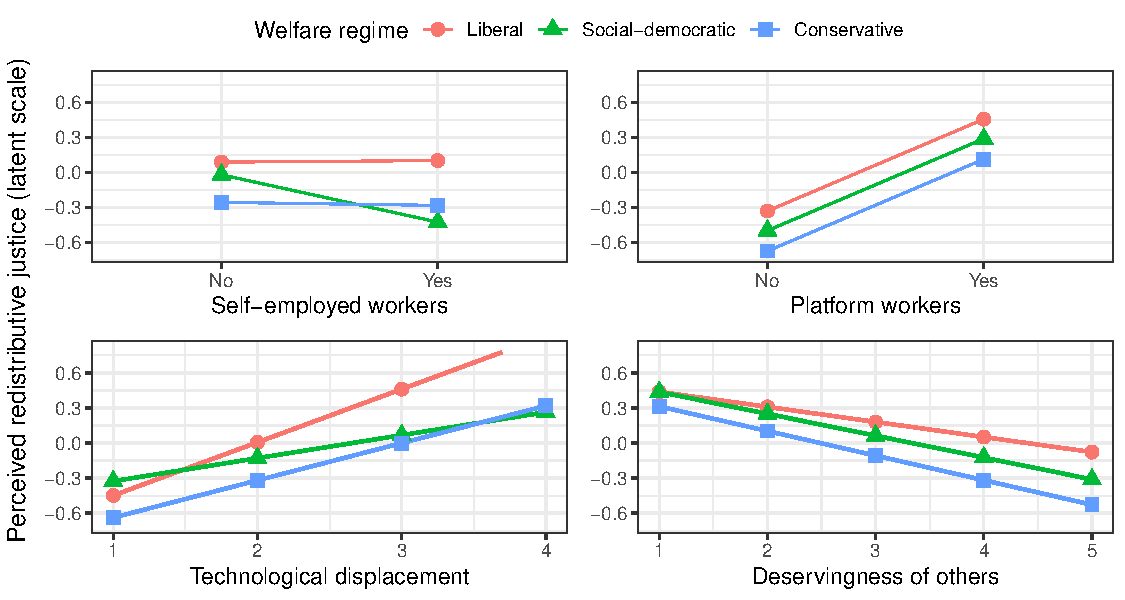
\includegraphics[width=0.85\linewidth,height=\textheight,keepaspectratio]{paper_files/figure-pdf/fig-interact-1.pdf}

}

\end{figure}%

emmip no estima probabilidades predicha, estima un factor latente entre
los cuatro interceptos para estimar propensión latente hacia las
categorías altas de perceción de justicia redistributiva

\section{Conclusion}\label{conclusion}



Síntesis y proyecciones futuras.

\section{References}\label{references}

\protect\phantomsection\label{refs}
\begin{CSLReferences}{1}{0}
\bibitem[\citeproctext]{ref-aidukaite_welfare_2011}
Aidukaite, J., 2011. Welfare reforms and socio-economic trends in the 10
new {EU} member states of {Central} and {Eastern Europe}. Communist and
Post-Communist Studies 44, 211--219.
\url{https://doi.org/10.1016/j.postcomstud.2011.07.005}

\bibitem[\citeproctext]{ref-anderson_workers_2007}
Anderson, C.J., Pontusson, J., 2007. Workers, worries and welfare
states: {Social} protection and job insecurity in 15 {OECD} countries.
European Journal of Political Research 46, 211--235.
\url{https://doi.org/10.1111/j.1475-6765.2007.00692.x}

\bibitem[\citeproctext]{ref-arntz_risk_2016}
Arntz, M., Gregory, T., Zierahn, U., 2016. The {Risk} of {Automation}
for {Jobs} in {OECD Countries}: {A Comparative Analysis} (\{\{OECD
Social\}\}, \{\{Employment\}\} and \{\{Migration Working Papers\}\} No.
189), {OECD Social}, {Employment} and {Migration Working Papers}.
\url{https://doi.org/10.1787/5jlz9h56dvq7-en}

\bibitem[\citeproctext]{ref-arts_three_2002}
Arts, W., Gelissen, J., 2002. Three worlds of welfare capitalism or
more? {A} state-of-the-art report. Journal of European Social Policy 12,
137--158. \url{https://doi.org/10.1177/0952872002012002114}

\bibitem[\citeproctext]{ref-autor_why_2015}
Autor, D.H., 2015. Why {Are There Still So Many Jobs}? {The History} and
{Future} of {Workplace Automation}. Journal of Economic Perspectives 29,
3--30. \url{https://doi.org/10.1257/jep.29.3.3}

\bibitem[\citeproctext]{ref-bambra_sifting_2007}
Bambra, C., 2007. {``{Sifting} the {Wheat} from the {Chaff}''}: {A
Two}-dimensional {Discriminant Analysis} of {Welfare State Regime
Theory}. Social Policy \& Administration 41, 1--28.
\url{https://doi.org/10.1111/j.1467-9515.2007.00536.x}

\bibitem[\citeproctext]{ref-behrendt_social_2019}
Behrendt, C., Nguyen, Q.A., Rani, U., 2019. Social protection systems
and the future of work: {Ensuring} social security for digital platform
workers. International Social Security Review 72, 17--41.
\url{https://doi.org/10.1111/issr.12212}

\bibitem[\citeproctext]{ref-blekesaune_public_2003}
Blekesaune, M., 2003. Public {Attitudes} toward {Welfare State
Policies}: {A Comparative Analysis} of 24 {Nations}. European
Sociological Review 19, 415--427.
\url{https://doi.org/10.1093/esr/19.5.415}

\bibitem[\citeproctext]{ref-brougham_smart_2018}
Brougham, D., Haar, J., 2018. Smart {Technology}, {Artificial
Intelligence}, {Robotics}, and {Algorithms} ({STARA}): {Employees}'
perceptions of our future workplace. Journal of Management \&
Organization 24, 239--257. \url{https://doi.org/10.1017/jmo.2016.55}

\bibitem[\citeproctext]{ref-busemeyer_social_2022}
Busemeyer, M.R., Sahm, A.H.J., 2022. Social {Investment},
{Redistribution} or {Basic Income}? {Exploring} the {Association Between
Automation Risk} and {Welfare State Attitudes} in {Europe}. Journal of
Social Policy 51, 751--770.
\url{https://doi.org/10.1017/S0047279421000519}

\bibitem[\citeproctext]{ref-bustelo_automation_2020}
Bustelo, M., Egaña Del Sol, P., Ripani, L., Soler, N., Viollaz, M.,
2020. Automation in {Latin America}: {Are Women} at {Higher Risk} of
{Losing Their Jobs}? Inter-American Development Bank.
\url{https://doi.org/10.18235/0002566}

\bibitem[\citeproctext]{ref-castillo_perception_2022}
Castillo, J.-C., García-Castro, J.-D., Venegas, M., 2022. Perception of
economic inequality: Concepts, associated factors and prospects of a
burgeoning research agenda ({Percepción} de desigualdad económica:
Conceptos, factores asociados y proyecciones de una agenda creciente de
investigación). International Journal of Social Psychology: Revista de
Psicología Social 37, 180--207.
\url{https://doi.org/10.1080/02134748.2021.2009275}

\bibitem[\citeproctext]{ref-castillo_perceptions_2025}
Castillo, J.C., Laffert, A., Carrasco, K., Iturra-Sanhueza, J., 2025.
Perceptions of inequality and meritocracy: Their interplay in shaping
preferences for market justice in {Chile} (2016--2023). Frontiers in
Sociology 10, 1634219. \url{https://doi.org/10.3389/fsoc.2025.1634219}

\bibitem[\citeproctext]{ref-cavaille_fair_2025}
Cavaillé, C., 2025. Fair {Enough}?: {Support} for {Redistribution} in
the {Age} of {Inequality}, 1st ed. Cambridge University Press.
\url{https://doi.org/10.1017/9781009366038}

\bibitem[\citeproctext]{ref-chung_institutions_2011}
Chung, H., Van Oorschot, W., 2011. Institutions versus market forces:
{Explaining} the employment insecurity of {European} individuals during
(the beginning of) the financial crisis. Journal of European Social
Policy 21, 287--301. \url{https://doi.org/10.1177/0958928711412224}

\bibitem[\citeproctext]{ref-cusack_risks_2006}
Cusack, T., Iversen, T., Rehm, P., 2006. Risks at {Work}: {The Demand}
and {Supply Sides} of {Government Redistribution}. Oxford Review of
Economic Policy 22, 365--389. \url{https://doi.org/10.1093/oxrep/grj022}

\bibitem[\citeproctext]{ref-dewitte_job_2005}
De Witte, H., 2005. Job insecurity: {Review} of the international
literature on definitions, prevalence, antecedents and consequences. SA
Journal of Industrial Psychology 31.
\url{https://doi.org/10.4102/sajip.v31i4.200}

\bibitem[\citeproctext]{ref-dekker_fear_2017}
Dekker, F., Salomons, A., Waal, J.V.D., 2017. Fear of robots at work:
The role of economic self-interest. Socio-Economic Review 15, 539--562.
\url{https://doi.org/10.1093/ser/mwx005}

\bibitem[\citeproctext]{ref-emmenegger_age_2012}
Emmenegger, P., Häusermann, S., Palier, B., Seeleib-Kaiser, M., 2012.
The age of dualization : The changing face of inequality in
deindustrializing societies. Oxford University Press.
\url{https://doi.org/10.5167/UZH-65793}

\bibitem[\citeproctext]{ref-esping-andersen_three_1993}
Esping-Andersen, G., 1993. The three worlds of welfare capitalism.
Polity press, Cambridge.

\bibitem[\citeproctext]{ref-fan_how_2024}
Fan, Z., Ning, J., He, A.J., 2024. How {Does Automation Risk Shape
Social Policy Preference}? {Employment Insecurity} and {Policy Feedback
Effect} in {China}. Social Policy and Society 23, 750--768.
\url{https://doi.org/10.1017/S1474746422000513}

\bibitem[\citeproctext]{ref-Fenger2006WelfareRI}
Fenger, H.J.M., 2006. Welfare regimes in central and eastern europe:
{Incorporating} post-communist countries in a welfare regime typology.

\bibitem[\citeproctext]{ref-ferrera_southern_1996}
Ferrera, M., 1996. The '{Southern Model}' of {Welfare} in {Social
Europe}. Journal of European Social Policy 6, 17--37.
\url{https://doi.org/10.1177/095892879600600102}

\bibitem[\citeproctext]{ref-finseraas_income_2009}
Finseraas, H., 2009. Income {Inequality} and {Demand} for
{Redistribution}: {A Multilevel Analysis} of {European Public Opinion}.
Scandinavian Political Studies 32, 94--119.
\url{https://doi.org/10.1111/j.1467-9477.2008.00211.x}

\bibitem[\citeproctext]{ref-frey_future_2017}
Frey, C.B., Osborne, M.A., 2017. The future of employment: {How}
susceptible are jobs to computerisation? Technological Forecasting and
Social Change 114, 254--280.
\url{https://doi.org/10.1016/j.techfore.2016.08.019}

\bibitem[\citeproctext]{ref-gallego_automation_2022}
Gallego, A., Kurer, T., 2022. Automation, {Digitalization}, and
{Artificial Intelligence} in the {Workplace}: {Implications} for
{Political Behavior}. Annual Review of Political Science 25, 463--484.
\url{https://doi.org/10.1146/annurev-polisci-051120-104535}

\bibitem[\citeproctext]{ref-gallie_economic_2013}
Gallie, D. (Ed.), 2013. Economic {Crisis}, {Quality} of {Work}, and
{Social Integration}: {The European Experience}. Oxford University
Press. \url{https://doi.org/10.1093/acprof:oso/9780199664719.001.0001}

\bibitem[\citeproctext]{ref-garcia-castro_perceiving_2020}
García-Castro, J.D., Rodríguez-Bailón, R., Willis, G.B., 2020.
Perceiving economic inequality in everyday life decreases tolerance to
inequality. Journal of Experimental Social Psychology 90, 104019.
\url{https://doi.org/10.1016/j.jesp.2020.104019}

\bibitem[\citeproctext]{ref-garcia-sanchez_attitudes_2020}
García-Sánchez, E., Osborne, D., Willis, G.B., Rodríguez-Bailón, R.,
2020. Attitudes towards redistribution and the interplay between
perceptions and beliefs about inequality. British Journal of Social
Psychology 59, 111--136. \url{https://doi.org/10.1111/bjso.12326}

\bibitem[\citeproctext]{ref-gimpelson_misperceiving_2018}
Gimpelson, V., Treisman, D., 2018. Misperceiving inequality. Economics
\& Politics 30, 27--54. \url{https://doi.org/10.1111/ecpo.12103}

\bibitem[\citeproctext]{ref-gutierrezcrocco_effects_2022}
Gutiérrez Crocco, F., Atzeni, M., 2022. The effects of the pandemic on
gig economy couriers in {Argentina} and {Chile}: {Precarity},
algorithmic control and mobilization. International Labour Review 161,
441--461. \url{https://doi.org/10.1111/ilr.12376}

\bibitem[\citeproctext]{ref-haubo_cumulative_2018}
Haubo, R., Christensen, B., 2018. Cumulative link models for ordinal
regression with the {R} package ordinal.

\bibitem[\citeproctext]{ref-howcroft_digitalisation_2025}
Howcroft, D., Banister, E., Jarvis-King, L., Rubery, J., Távora, I.,
2025. Digitalisation and the {Remaking} of the {Ideal Worker}. Work,
Employment and Society 39, 703--726.
\url{https://doi.org/10.1177/09500170241301015}

\bibitem[\citeproctext]{ref-hox_multilevel_2017}
Hox, J.J., Moerbeek, M., Van De Schoot, R., 2017. Multilevel {Analysis}:
{Techniques} and {Applications}, 3rd ed. Routledge, Third edition.
\textbar{} New York, NY : Routledge, 2017.\textbar
\url{https://doi.org/10.4324/9781315650982}

\bibitem[\citeproctext]{ref-im_losers_2019}
Im, Z.J., Mayer, N., Palier, B., Rovny, J., 2019. The {``losers of
automation''}: {A} reservoir of votes for the radical right? Research \&
Politics 6, 2053168018822395.
\url{https://doi.org/10.1177/2053168018822395}

\bibitem[\citeproctext]{ref-iversen_asset_2001}
Iversen, T., Soskice, D., 2001. An {Asset Theory} of {Social Policy
Preferences}. American Political Science Review 95, 875--893.
\url{https://doi.org/10.1017/S0003055400400079}

\bibitem[\citeproctext]{ref-jaeger_welfare_2006}
Jæger, M.M., 2006. Welfare {Regimes} and {Attitudes Towards
Redistribution}: {The Regime Hypothesis Revisited}. European
Sociological Review 22, 157--170.
\url{https://doi.org/10.1093/esr/jci049}

\bibitem[\citeproctext]{ref-kalleberg_good_2011}
Kalleberg, A., 2011. Good jobs, bad jobs: {The} rise of polarized and
precarious employment systems in the {United States}, 1970s-2000s, Good
Jobs, Bad Jobs: The Rise of Polarized and Precarious Employment Systems
in the United States, 1970s-2000s.

\bibitem[\citeproctext]{ref-kenworthy_inequality_2007}
Kenworthy, L., McCall, L., 2007. Inequality, public opinion and
redistribution. Socio-Economic Review 6, 35--68.
\url{https://doi.org/10.1093/ser/mwm006}

\bibitem[\citeproctext]{ref-korpi_paradox_1998}
Korpi, W., Palme, J., 1998. The {Paradox} of {Redistribution} and
{Strategies} of {Equality}: {Welfare State Institutions}, {Inequality},
and {Poverty} in the {Western Countries}. American Sociological Review
63, 661. \url{https://doi.org/10.2307/2657333}

\bibitem[\citeproctext]{ref-kurer_declining_2020}
Kurer, T., 2020. The {Declining Middle}: {Occupational Change}, {Social
Status}, and the {Populist Right}. Comparative Political Studies 53,
1798--1835. \url{https://doi.org/10.1177/0010414020912283}

\bibitem[\citeproctext]{ref-laenen_welfare_2020}
Laenen, T., 2020. Welfare deservingness and welfare policy: Popular
deservingness opinions and their interaction with welfare state
policies. Edward Elgar Publishing, Cheltenham, UK Northampton, MA, USA.

\bibitem[\citeproctext]{ref-larsen_institutional_2008}
Larsen, C.A., 2008. The {Institutional Logic} of {Welfare Attitudes}:
{How Welfare Regimes Influence Public Support}. Comparative Political
Studies 41, 145--168. \url{https://doi.org/10.1177/0010414006295234}

\bibitem[\citeproctext]{ref-lenth_emmeans_2017}
Lenth, R.V., Piaskowski, J., 2017. Emmeans: {Estimated Marginal Means},
aka {Least-Squares Means}.
\url{https://doi.org/10.32614/CRAN.package.emmeans}

\bibitem[\citeproctext]{ref-lindh_class_2020}
Lindh, A., McCall, L., 2020. Class {Position} and {Political Opinion} in
{Rich Democracies}. Annual Review of Sociology 46, 419--441.
\url{https://doi.org/10.1146/annurev-soc-121919-054609}

\bibitem[\citeproctext]{ref-franzoni_welfare_2008}
Martínez Franzoni, J., 2008. Welfare {Regimes} in {Latin America}:
{Capturing Constellations} of {Markets}, {Families}, and {Policies}.
Latin American Politics and Society 50, 67--100.
\url{https://doi.org/10.1111/j.1548-2456.2008.00013.x}

\bibitem[\citeproctext]{ref-marx_effect_2014}
Marx, P., 2014. The effect of job insecurity and employability on
preferences for redistribution in {Western Europe}. Journal of European
Social Policy 24, 351--366.
\url{https://doi.org/10.1177/0958928714538217}

\bibitem[\citeproctext]{ref-mau_moral_2014}
Mau, S., 2014. The moral economy of welfare states: {Britain} and
{Germany} compared, First issued in paperback. ed, Routledge/{EUI}
studies in the political economy of welfare. Routledge \& Francis Group,
London New York NY.

\bibitem[\citeproctext]{ref-mccall_undeserving_2013}
McCall, L., 2013. The {Undeserving Rich}: {American Beliefs} about
{Inequality}, {Opportunity}, and {Redistribution}, 1st ed. Cambridge
University Press. \url{https://doi.org/10.1017/CBO9781139225687}

\bibitem[\citeproctext]{ref-mijs_paradox_2021}
Mijs, J.J.B., 2021. The paradox of inequality: Income inequality and
belief in meritocracy go hand in hand. Socio-Economic Review 19, 7--35.
\url{https://doi.org/10.1093/ser/mwy051}

\bibitem[\citeproctext]{ref-osberg_fair_2006}
Osberg, L., Smeeding, T., 2006. {``{Fair}''} {Inequality}? {Attitudes}
toward {Pay Differentials}: {The United States} in {Comparative
Perspective}. American Sociological Review 71, 450--473.
\url{https://doi.org/10.1177/000312240607100305}

\bibitem[\citeproctext]{ref-perez_building_2023}
Pérez-Ahuamda, P., 2023. Building power to shape labor policy: Unions,
employer associations, and reform in neoliberal {Chile}, Pitt {Latin
American} series. University of Pittsburgh Press, Pittsburgh (Pa.).

\bibitem[\citeproctext]{ref-perez-ahumada_conditioning_2026}
Pérez-Ahumada, P., Olivares-Collío, D., Carrasco, K., 2026. The
conditioning power of class: {Collective} action and attitudes toward
inequality in neoliberal {Chile} (2016--2023). Critical Sociology
08969205261417585. \url{https://doi.org/10.1177/08969205261417585}

\bibitem[\citeproctext]{ref-petersen_social_2012}
Petersen, M.B., 2012. Social {Welfare} as {Small}-{Scale Help}:
{Evolutionary Psychology} and the {Deservingness Heuristic}. American
Journal of Political Science 56, 1--16.
\url{https://doi.org/10.1111/j.1540-5907.2011.00545.x}

\bibitem[\citeproctext]{ref-reeskens_equity_2013}
Reeskens, T., Van Oorschot, W., 2013. Equity, equality, or need? {A}
study of popular preferences for welfare redistribution principles
across 24 {European} countries. Journal of European Public Policy 20,
1174--1195. \url{https://doi.org/10.1080/13501763.2012.752064}

\bibitem[\citeproctext]{ref-rehm_risks_2009}
Rehm, P., 2009. Risks and {Redistribution}: {An Individual-Level
Analysis}. Comparative Political Studies 42, 855--881.
\url{https://doi.org/10.1177/0010414008330595}

\bibitem[\citeproctext]{ref-roosma_just_2016}
Roosma, F., Van Oorschot, W., Gelissen, J., 2016. A {Just Distribution}
of {Burdens}? {Attitudes Toward} the {Social Distribution} of {Taxes} in
26 {Welfare States}. International Journal of Public Opinion Research
28, 376--400. \url{https://doi.org/10.1093/ijpor/edv020}

\bibitem[\citeproctext]{ref-rothstein_just_1998}
Rothstein, B., 1998. Just {Institutions Matter}: {The Moral} and
{Political Logic} of the {Universal Welfare State}, 1st ed. Cambridge
University Press. \url{https://doi.org/10.1017/CBO9780511598449}

\bibitem[\citeproctext]{ref-rueda_social_2007}
Rueda, D., 2007. Social {Democracy Inside Out}: {Partisanship} and
{Labor Market Policy} in {Advanced Industrialized Democracies}, 1st ed.
Oxford University PressOxford.
\url{https://doi.org/10.1093/acprof:oso/9780199216352.001.0001}

\bibitem[\citeproctext]{ref-schmidt-catran_economic_2016}
Schmidt-Catran, A.W., 2016. Economic inequality and public demand for
redistribution: Combining cross-sectional and longitudinal evidence.
Socio-Economic Review 14, 119--140.
\url{https://doi.org/10.1093/ser/mwu030}

\bibitem[\citeproctext]{ref-schor_gig_2020}
Schor, J.B., 2020. After the gig: How the sharing economy got hijacked
and how to win it back. University of California Press, Oakland,
California.

\bibitem[\citeproctext]{ref-schwander_who_2013}
Schwander, H., Häusermann, S., 2013. Who is in and who is out? {A}
risk-based conceptualization of insiders and outsiders. Journal of
European Social Policy 23, 248--269.
\url{https://doi.org/10.1177/0958928713480064}

\bibitem[\citeproctext]{ref-snijders_multilevel_2012}
Snijders, T.A.B., Bosker, R.J., 2012. Multilevel analysis: An
introduction to basic and advanced multilevel modeling, 2nd ed. ed.
Sage, Los Angeles.

\bibitem[\citeproctext]{ref-standing_precariat_2014}
Standing, G., 2014. The precariat: The new dangerous class. Bloomsbury,
London, UK ; New York, NY.

\bibitem[\citeproctext]{ref-svallfors_government_2013}
Svallfors, S., 2013. Government quality, egalitarianism, and attitudes
to taxes and social spending: A {European} comparison. European
Political Science Review 5, 363--380.
\url{https://doi.org/10.1017/S175577391200015X}

\bibitem[\citeproctext]{ref-svallfors_worlds_1997}
Svallfors, S., 1997. Worlds of {Welfare} and {Attitudes} to
{Redistribution}: {A Comparison} of {Eight Western Nations}. European
Sociological Review 13, 283--304.
\url{https://doi.org/10.1093/oxfordjournals.esr.a018219}

\bibitem[\citeproctext]{ref-sverke_no_2002}
Sverke, M., Hellgren, J., Näswall, K., 2002. No security: {A}
meta-analysis and review of job insecurity and its consequences. Journal
of Occupational Health Psychology 7, 242--264.
\url{https://doi.org/10.1037/1076-8998.7.3.242}

\bibitem[\citeproctext]{ref-thewissen_automation_2019}
Thewissen, S., Rueda, D., 2019. Automation and the {Welfare State}:
{Technological Change} as a {Determinant} of {Redistribution
Preferences}. Comparative Political Studies 52, 171--208.
\url{https://doi.org/10.1177/0010414017740600}

\bibitem[\citeproctext]{ref-vallas_what_2020}
Vallas, S., Schor, J.B., 2020. What {Do Platforms Do}? {Understanding}
the {Gig Economy}. Annual Review of Sociology 46, 273--294.
\url{https://doi.org/10.1146/annurev-soc-121919-054857}

\bibitem[\citeproctext]{ref-vanoorschot_making_2006}
Van Oorschot, W., 2006. Making the difference in social {Europe}:
Deservingness perceptions among citizens of {European} welfare states.
Journal of European Social Policy 16, 23--42.
\url{https://doi.org/10.1177/0958928706059829}

\bibitem[\citeproctext]{ref-oorschot_who_2000}
Van Oorschot, W., 2000. Who should get what, and why? {On} deservingness
criteria and the conditionality of solidarity among the public. Policy
\& Politics 28, 33--48. \url{https://doi.org/10.1332/0305573002500811}

\bibitem[\citeproctext]{ref-vanoorschot_social_2017}
Van Oorschot, W., Roosma, F., Meuleman, B., Reeskens, T. (Eds.), 2017.
The {Social Legitimacy} of {Targeted Welfare}: {Attitudes} to {Welfare
Deservingness}. Edward Elgar Publishing.
\url{https://doi.org/10.4337/9781785367212}

\bibitem[\citeproctext]{ref-wood_good_2019}
Wood, A.J., Graham, M., Lehdonvirta, V., Hjorth, I., 2019. Good {Gig},
{Bad Gig}: {Autonomy} and {Algorithmic Control} in the {Global Gig
Economy}. Work, Employment and Society 33, 56--75.
\url{https://doi.org/10.1177/0950017018785616}

\end{CSLReferences}




\end{document}
